\begin{figure}[H]
	\begin{subfigure}{0.5\textwidth}
		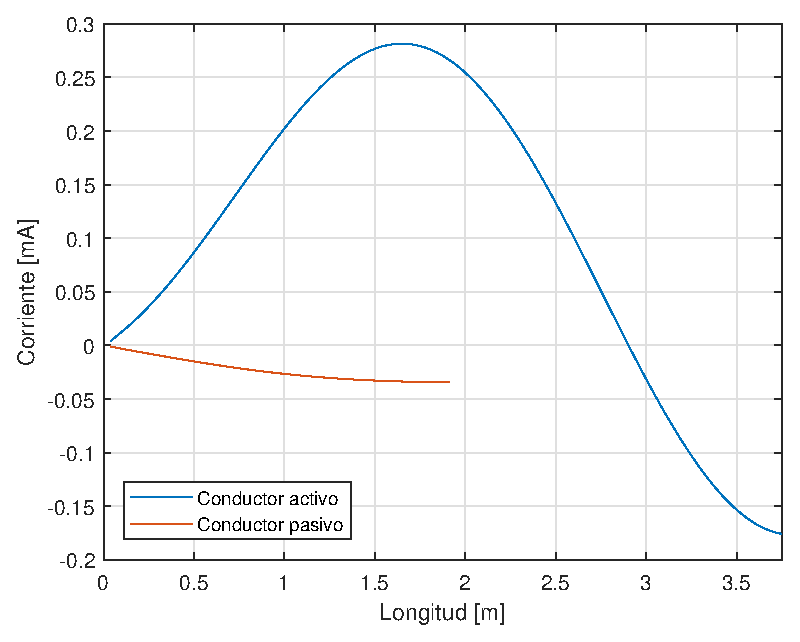
\includegraphics[scale=0.6]{imagenes/i_real_80_tierra.eps}
		\caption{Parte real.}
		\label{fig.i_real_80_tierra}
	\end{subfigure}
	\quad
	\begin{subfigure}{0.5\textwidth}
		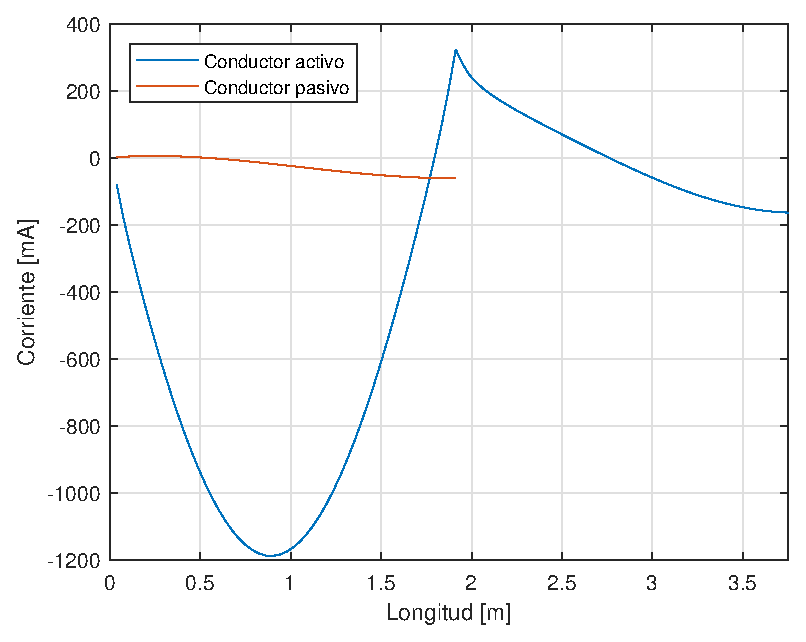
\includegraphics[scale=0.6]{imagenes/i_imag_80_tierra.eps}
		\caption{Parte imaginaria.}
		\label{fig.i_imag_80_tierra}
	\end{subfigure}
	\quad
	\begin{subfigure}{0.5\textwidth}
		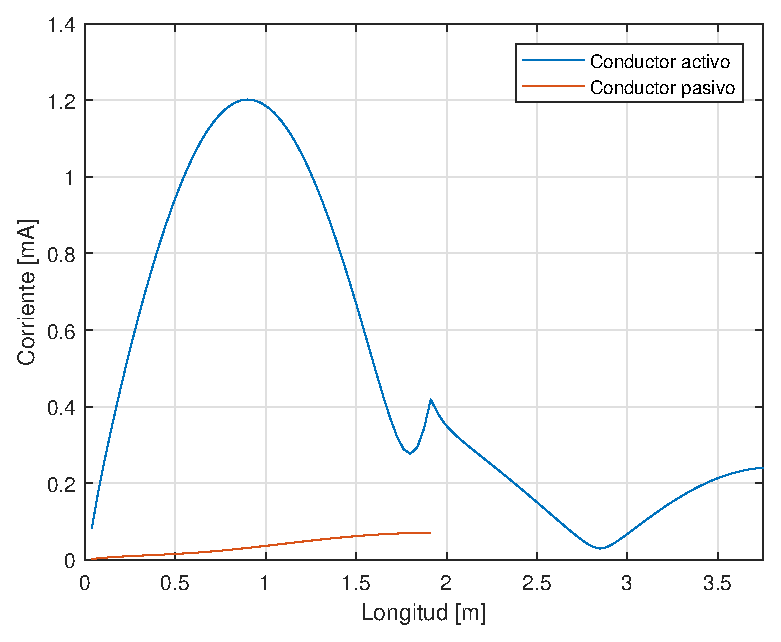
\includegraphics[scale=0.6]{imagenes/i_mag_80_tierra.eps}
		\caption{Magnitud.}
		\label{fig.i_mag_80_tierra}
	\end{subfigure}
	\quad
	\begin{subfigure}{0.5\textwidth}
		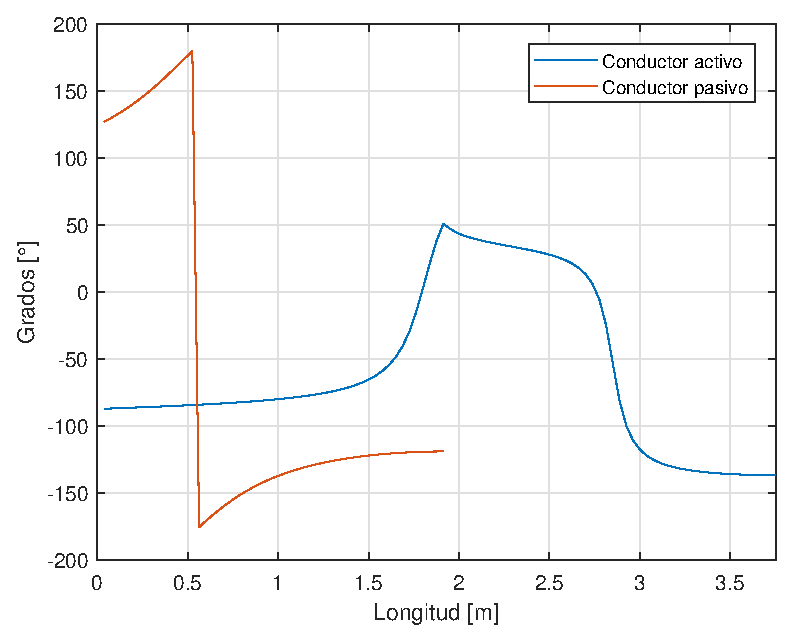
\includegraphics[scale=0.6]{imagenes/i_fase_80_tierra.eps}
		\caption{Fase.}
		\label{fig.i_fase_80_tierra}
	\end{subfigure}
	\caption{Corriente para la frecuencia mínima $f = \SI{80}{\mega\hertz}$}
\end{figure}

\begin{figure}[H]
	\begin{subfigure}{0.5\textwidth}
		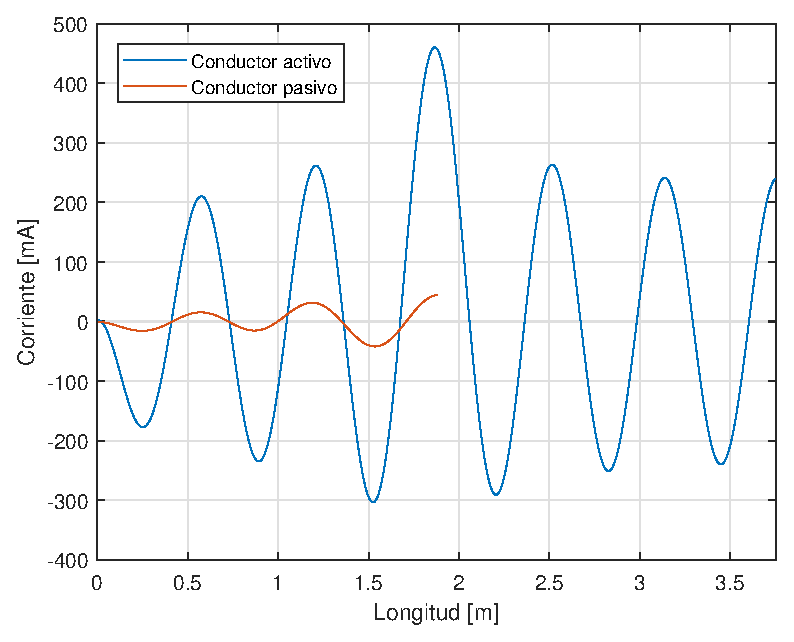
\includegraphics[scale=0.6]{imagenes/i_real_480_tierra.eps}
		\caption{Parte real.}
		\label{fig.i_real_480_tierra}
	\end{subfigure}
	\quad
	\begin{subfigure}{0.5\textwidth}
		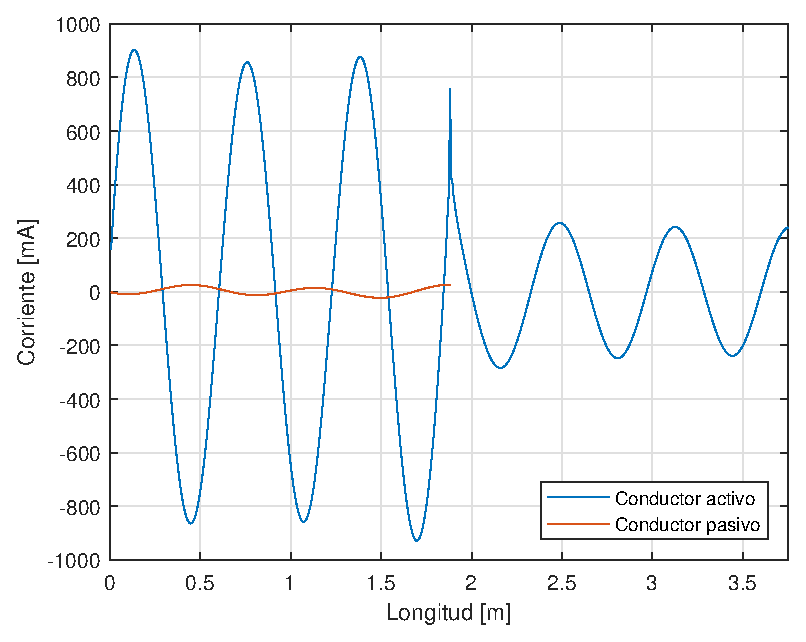
\includegraphics[scale=0.6]{imagenes/i_imag_480_tierra.eps}
		\caption{Parte imaginaria.}
		\label{fig.i_imag_480_tierra}
	\end{subfigure}
	\quad
	\begin{subfigure}{0.5\textwidth}
		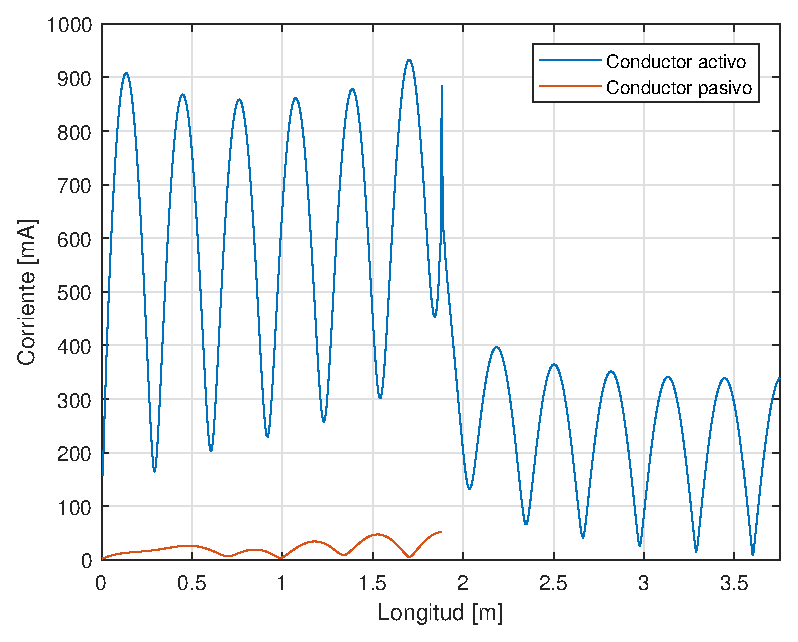
\includegraphics[scale=0.6]{imagenes/i_mag_480_tierra.eps}
		\caption{Magnitud.}
		\label{fig.i_mag_480_tierra}
	\end{subfigure}
	\quad
	\begin{subfigure}{0.5\textwidth}
		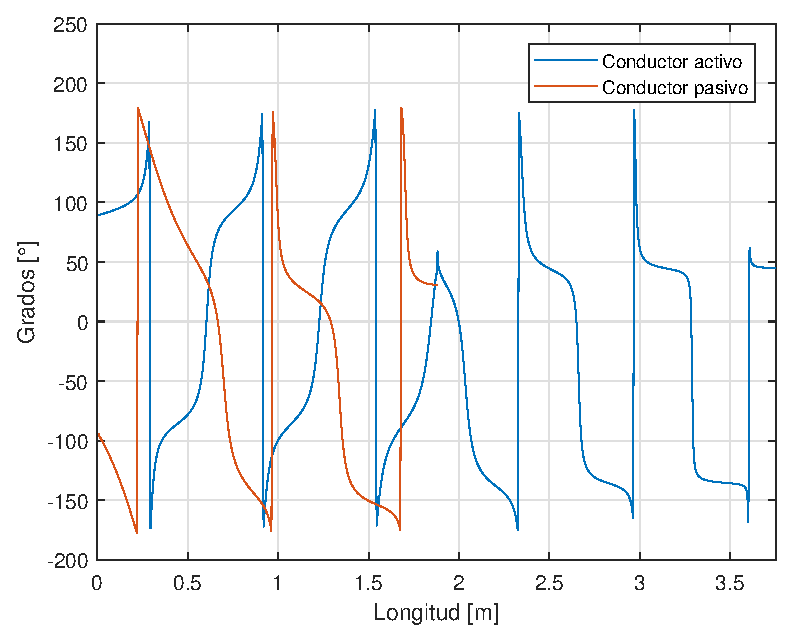
\includegraphics[scale=0.6]{imagenes/i_fase_480_tierra.eps}
		\caption{Fase.}
		\label{fig.i_fase_480_tierra}
	\end{subfigure}
	\caption{Corriente para la frecuencia máxima $f = \SI{480}{\mega\hertz}$}
\end{figure}

Al comparar las figuras \ref{fig.i_mag_480} y \ref{fig.i_mag_480_tierra} de magnitud se observa que el segundo máximo de corriente del caso espacio libre se atenúa al anexar el plano de tierra. En el caso del gráfico de fase, en este caso el conductor pasivo a mitad de su longitud cambia de fase, siendo opuesta a la fase del inicio.
Para ambas frecuencias, se produce el mismo efecto al agregar el plano de tierra, la magnitud de la corriente tiende a disminuir hacia el extremo superior del conductor activo.
